\documentclass[tikz,border=5pt]{standalone}
\usepackage{tikz}
\usetikzlibrary{positioning,arrows.meta,calc,fit,backgrounds}
\usepackage{amsmath}

\definecolor{convcolor}{RGB}{100,149,237}    % cornflower blue
\definecolor{bncolor}{RGB}{144,238,144}      % light green
\definecolor{actcolor}{RGB}{255,179,71}      % pastel orange
\definecolor{poolcolor}{RGB}{221,160,221}    % plum
\definecolor{headcolor}{RGB}{255,218,185}    % peach puff
\definecolor{inputcolor}{RGB}{211,211,211}   % light grey
\definecolor{outputcolor}{RGB}{255,255,224}  % light yellow

\newcommand{\opbox}[4][]{%
  % #1 = optional tikz args
  % #2 = width
  % #3 = height
  % #4 = content
  \node[#1,minimum width=#2,minimum height=#3,inner sep=1pt,font=\tiny,align=center] {#4}%
}

\begin{document}
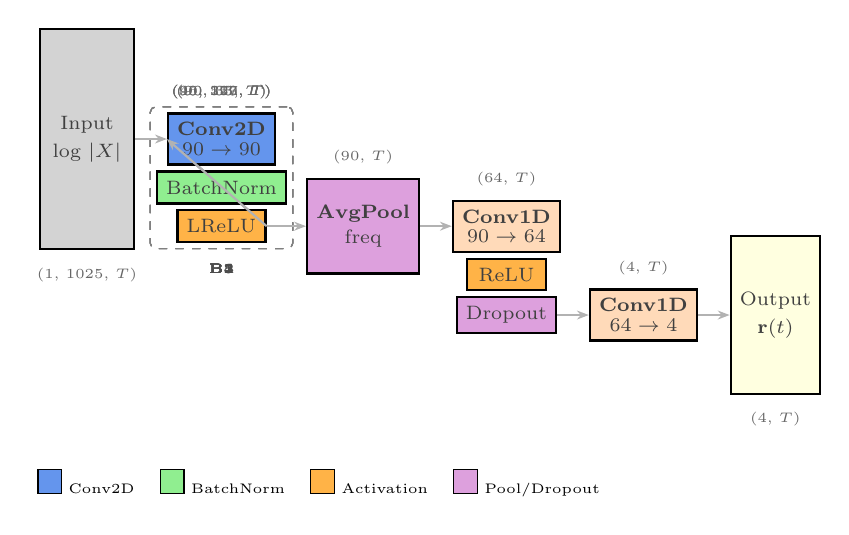
\begin{tikzpicture}[
  node distance=0.8mm and 3mm,
  arr/.style={-{Stealth[length=1.5mm]},thick,draw=gray!60},
  labelnode/.style={font=\scriptsize,align=center,text=darkgray},
  dimlabel/.style={font=\tiny,align=center,text=gray!80!black},
]

% --- INPUT ---
\node[fill=inputcolor,draw=black,thick,minimum width=1.2cm,minimum height=2.8cm,labelnode] (input)
  {Input\\[2pt]log $|X|$};
\node[dimlabel,below=1mm of input] {(1, 1025, $T$)};

% Helper macro for a single encoder block
\def\encoderblock#1#2#3#4#5{%
  % #1=anchor node to place after
  % #2=channels in
  % #3=channels out
  % #4=kernel
  % #5=freq out
  \node[fill=convcolor,draw=black,thick,minimum width=1.0cm,minimum height=0.55cm,right=4mm of #1,labelnode]
    (#1conv) {\textbf{Conv2D}\\[-1pt]$#2\to#3$};
  \node[fill=bncolor,draw=black,thick,minimum width=1.0cm,minimum height=0.35cm,below=0.6mm of #1conv,labelnode]
    (#1bn) {BatchNorm};
  \node[fill=actcolor,draw=black,thick,minimum width=1.0cm,minimum height=0.35cm,below=0.6mm of #1bn,labelnode]
    (#1act) {LReLU};
  \node[dimlabel,above=0.5mm of #1conv] {($#3$, #5, $T$)};
}

% --- BLOCK 1 ---
\encoderblock{input}{1}{45}{7\times5}{513}
\draw[arr] (input.east) -- (inputconv.west);

% --- BLOCK 2 ---
\encoderblock{input}{45}{90}{7\times5}{257}
\draw[arr] (inputact.east) -- (inputconv.west);

% --- BLOCK 3 ---
\encoderblock{input}{90}{90}{5\times3}{129}
\draw[arr] (inputact.east) -- (inputconv.west);

% --- BLOCK 4 ---
\encoderblock{input}{90}{90}{5\times3}{65}
\draw[arr] (inputact.east) -- (inputconv.west);

% --- BLOCK 5 ---
\encoderblock{input}{90}{90}{5\times3}{33}
\draw[arr] (inputact.east) -- (inputconv.west);

% Rename the last block's nodes for clarity
\node[inner sep=0] (b5conv) at (inputconv) {};
\node[inner sep=0] (b5bn)   at (inputbn)   {};
\node[inner sep=0] (b5act)  at (inputact)  {};

% --- SPATIAL AVERAGE POOL ---
\node[fill=poolcolor,draw=black,thick,minimum width=1.0cm,minimum height=1.2cm,right=5mm of inputact,labelnode]
  (pool) {\textbf{AvgPool}\\[1pt]freq};
\node[dimlabel,above=0.5mm of pool] {(90, $T$)};
\draw[arr] (inputact.east) -- (pool.west);

% --- HEAD: Conv1D 90->64 ---
\node[fill=headcolor,draw=black,thick,minimum width=1.0cm,minimum height=0.55cm,right=4mm of pool,labelnode]
  (h1) {\textbf{Conv1D}\\[-1pt]$90\to64$};
\node[fill=actcolor,draw=black,thick,minimum width=1.0cm,minimum height=0.35cm,below=0.6mm of h1,labelnode]
  (h1act) {ReLU};
\node[fill=poolcolor,draw=black,thick,minimum width=1.0cm,minimum height=0.35cm,below=0.6mm of h1act,labelnode]
  (h1drop) {Dropout};
\node[dimlabel,above=0.5mm of h1] {(64, $T$)};
\draw[arr] (pool.east) -- (h1.west);

% --- HEAD: Conv1D 64->4 ---
\node[fill=headcolor,draw=black,thick,minimum width=1.0cm,minimum height=0.55cm,right=4mm of h1drop,labelnode]
  (h2) {\textbf{Conv1D}\\[-1pt]$64\to4$};
\node[dimlabel,above=0.5mm of h2] {(4, $T$)};
\draw[arr] (h1drop.east) -- (h2.west);

% --- OUTPUT ---
\node[fill=outputcolor,draw=black,thick,minimum width=1.0cm,minimum height=2.0cm,right=4mm of h2,labelnode]
  (output) {Output\\[2pt]$\mathbf{r}(t)$};
\node[dimlabel,below=1mm of output] {(4, $T$)};
\draw[arr] (h2.east) -- (output.west);

% --- BRACE + BLOCK LABELS ---
\begin{scope}[on background layer]
  \node[draw=gray,dashed,rounded corners=2pt,inner sep=2pt,fit=(inputconv)(inputbn)(inputact)] (block1) {};
  \node[draw=gray,dashed,rounded corners=2pt,inner sep=2pt,fit=(inputconv)(inputbn)(inputact)] (block2) {};
  \node[draw=gray,dashed,rounded corners=2pt,inner sep=2pt,fit=(inputconv)(inputbn)(inputact)] (block3) {};
  \node[draw=gray,dashed,rounded corners=2pt,inner sep=2pt,fit=(inputconv)(inputbn)(inputact)] (block4) {};
  \node[draw=gray,dashed,rounded corners=2pt,inner sep=2pt,fit=(inputconv)(inputbn)(inputact)] (block5) {};
\end{scope}

% Block numbers below
\foreach \n/\t in {1/B1,2/B2,3/B3,4/B4,5/B5} {
  \node[font=\tiny\bfseries,text=gray!60!black] at ($(block\n.south)-(0,2.5mm)$) {\t};
}

% Legend
\node[anchor=north west,font=\tiny] at ($(current bounding box.south west)+(0,-3mm)$) {
  \tikz\node[fill=convcolor,draw,minimum size=3mm]{}; Conv2D \quad
  \tikz\node[fill=bncolor,draw,minimum size=3mm]{}; BatchNorm \quad
  \tikz\node[fill=actcolor,draw,minimum size=3mm]{}; Activation \quad
  \tikz\node[fill=poolcolor,draw,minimum size=3mm]{}; Pool/Dropout
};

\end{tikzpicture}
\end{document}
